\section{DP Framework}\label{DP Framework}

We first recapitulate dependency pairs for ordinary (non-relative) rewriting in \Cref{Dependency Pairs for Ordinary Term Rewriting}
and summarize existing results on DPs for relative rewriting in \Cref{Dependency Pairs for Relative Termination}.

\subsection{Dependency Pairs for Ordinary Term Rewriting}\label{Dependency Pairs for Ordinary Term Rewriting}

We recapitulate DPs and the two most important processors of the DP framework, and refer to, e.g.,
\cite{arts2000termination,gieslLPAR04dpframework,giesl2006mechanizing,hirokawa2005automating,DBLP:journals/iandc/HirokawaM07}
for more details.
As an example, we show how to prove termination of $\R_{\tdivl}$ without the base $\R^{=}_{\tset}$.
We decompose the signature
$\Sigma =  \SignatureC \uplus  \SignatureD$ of a TRS $\R$ 
such that $f \in \SignatureD$ if $f = \rootsym(\ell)$ for some rule $\ell \to r \in \R$.
The symbols in $\SignatureC$ and $\SignatureD$ are called 
\emph{constructors} and \emph{defined symbols} of $\R$, respectively. 
For every $f \in \SignatureD$, we introduce a fresh \emph{annotated symbol} $f^{\#}$ of the same arity.
Let $\SignatureA$ denote the set of all annotated symbols, and $\SignatureADC = \Sigma \uplus \SignatureA$.
To ease readability, we often use capital letters like $\tF$ instead of $\tf^\#$.
For any term $t = f(t_1,\ldots,t_n) \in \TSet{\Sigma}{\VSet}$ with $f \in \SignatureD$, 
let $t^{\#} = f^{\#}(t_1,\ldots,t_n)$.
For a rule $\ell \to r$ and each subterm $t$ of $r$ with \pagebreak[2] defined root symbol, one obtains a
\emph{dependency pair} $\ell^\# \to t^\#$.
Let $\DPair{\R}$ denote the set of all dependency pairs of the TRS $\R$.

\begin{example}
  \label{example:dependency-pair}
    For $\R_{\tdivl}$ from \Cref{ex:divlTRS}, we obtain the following five dependency pairs.

    \vspace*{-.5cm}
    
    {\footnotesize
    \hspace*{-.9cm}
    \begin{minipage}[t]{5.7cm}
             \begin{align}
          \label{R-div-deppair-3} \tM(\ts(x),\ts(y)) &\to \tM(x,y) \\
            \label{R-div-deppair-2} \tD(\ts(x),\ts(y)) &\to \tM(x,y) \\
           \label{R-div-deppair-1} \tD(\ts(x),\ts(y)) &\to \tD(\tm(x,y),\ts(y))        
            \end{align}
    \end{minipage}\hspace*{.3cm}
    \begin{minipage}[t]{6.6cm}
        \begin{align}
            \label{R-div-deppair-4} \tDL(x,\tcons(y,\xs)) &\to \tD(x,y) \\
            \label{R-div-deppair-5} \tDL(x,\tcons(y,\xs)) &\to \tDL(\tdiv(x,y),\xs) 
        \end{align}
    \end{minipage}}
\end{example}

The DP framework operates on \emph{DP problems} $(\C{P}, \R)$ where
$\C{P}$ is a (finite) set of DPs, and $\R$ is a (finite) TRS. 
A (possibly infinite) sequence $t_0, t_1, t_2,
\ldots$ with $t_i \rootto_{\C{P}} \circ \to_{\R}^* t_{i+1}$ for all $i$ is a $(\C{P}, \R)$-\emph{chain}.
Here, $\rootto$ denotes rewrite steps at the root.
Intuitively, a chain represents subsequent ``function calls''  in evaluations. 
Between two function calls (corres\-ponding to steps with $\C{P}$, called $\mathbf{p}$-steps) one can evaluate the
arguments using arbitrary many steps with $\R$ (called $\mathbf{r}$-steps).
So $\mathbf{r}$-steps are rewrite steps that are needed in order to enable another
$\mathbf{p}$-step at a position above later on.\linebreak
For example, $\tDL(\ts(\O), \tcons(\ts(\O), \tnil)), \tDL(\ts(\O),\tnil)$ is a
$(\DPair{\R_{\tdivl}}, \R_{\tdivl})$-chain, as $\tDL(\ts(\O), \tcons(\ts(\O), \tnil))
\rootto_{\DPair{\R_{\tdivl}}} \tDL(\tdiv(\ts(\O),\ts(\O)),\tnil) \to_{\R_{\tdivl}}^*\!\tDL(\ts(\O),\tnil)$.

A DP problem $(\C{P}, \R)$ is called
\emph{strongly normalizing (SN)} if there is no infinite $(\C{P}, \R)$-chain.
The main result on DPs is the \emph{chain criterion} which states that a TRS
$\R$ is SN iff $(\DPair{\R}, \R)$ is SN.
The key idea of the DP framework is a \emph{divide-and-conquer} approach which
applies \emph{DP processors} to transform DP problems into simpler sub-problems.
A \emph{DP processor} $\Proc$ has the form $\Proc(\C{P}, \R) = \{(\C{P}_1,\R_1), \ldots, (\C{P}_n,\R_n)\}$, 
where $\C{P}, \C{P}_1, \ldots, \C{P}_n$ are sets of DPs and $\R, \R_1, \ldots, \R_n$ are TRSs. 
$\Proc$ is \emph{sound} if $(\C{P}, \R)$ is SN whenever 
$(\C{P}_i,\R_i)$ is SN for all $1 \leq i \leq n$. 
It is \emph{complete} if $(\C{P}_i,\R_i)$ is SN for all 
$1 \leq i \leq n$ whenever $(\C{P}, \R)$ is SN.


So for a TRS $\R$, one starts with the initial
DP problem $(\DPair{\R}, \R)$ and applies sound 
(and preferably complete) DP processors until all sub-problems are ``solved'' (i.e.,
DP processors transform them to the empty set).
This allows for modular ter-\linebreak mination
proofs, as different techniques can be applied on each sub-problem $(\C{P}_i, \R_i)$.

One of the most important processors is the \emph{dependency graph processor}.
The \emph{$(\C{P}, \R)$-dependency graph} indicates
which DPs can be used after each other in  
chains.\linebreak
Its nodes are $\C{P}$ and there is an edge from $s_1 \to t_1$ to $s_2 \to t_2$ if there
are substitutions
\begin{wrapfigure}[5]{r}{0.14\textwidth}
  \begin{center}
  \scriptsize
    \vspace*{-1.3cm}
    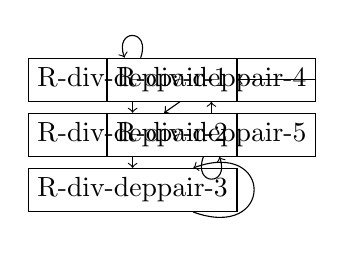
\begin{tikzpicture}
        \node[shape=rectangle,draw=black!100] (A) at (1,0.7) {\eqref{R-div-deppair-5}};
        \node[shape=rectangle,draw=black!100] (B) at (1,1.4) {\eqref{R-div-deppair-4}};
        \node[shape=rectangle,draw=black!100] (C) at (0,0) {\eqref{R-div-deppair-3}};
        \node[shape=rectangle,draw=black!100] (D) at (0,.7) {\eqref{R-div-deppair-2}};
        \node[shape=rectangle,draw=black!100] (E) at (0,1.4) {\eqref{R-div-deppair-1}};
   
        \path [->,in=290,out=250,looseness=5] (A) edge (A);
        \path [->] (A) edge (B);
        \path [->] (B) edge (D);
        \path [->] (B) edge (E);
        \path [->,in=20,out=340,looseness=5] (C) edge (C);
        \path [->] (D) edge (C);
        \path [->] (E) edge (D);
        \path [->,in=110,out=70,looseness=5] (E) edge (E);
    \end{tikzpicture}
    \caption*{}
  \end{center}
\end{wrapfigure}
$\sigma_1, \sigma_2$ with $t_1 \sigma_1 \to_{\R}^* s_2 \sigma_2$.
The $(\DPair{\R_{\tdivl}}, \R_{\tdivl})$-dependency graph is on the right.
Any infinite $(\C{P}, \R)$-chain corresponds to
an infinite path in the dependency graph, and since the graph is finite, this infinite
path must end in a strongly connected component (SCC).\footnote{Here, a
set $\C{P}'$ of dependency pairs is  an \emph{SCC} if it is a maximal cycle,
i.e., it is a maximal set such that for any $s_1 \to t_1$ and $s_2 \to
t_2$ in $\C{P}'$ there is
a non-empty path from $s_1 \to t_1$ to $s_2 \to
t_2$ which only traverses nodes from $\C{P}'$.}
Hence, it suffices to consider the SCCs of this graph independently.

\begin{restatable}[Dep.\ Graph Processor]{theorem}{depgraph}\label{DGP}
    For the SCCs $\C{P}_1, \ldots, \C{P}_n$ of the $(\C{P}, \R)$-dependency graph,  
    $\Proc_{\mathtt{DG}}(\C{P},\R) = \{(\C{P}_1,\R), \ldots, (\C{P}_n,\R)\}$ is sound and complete. 
\end{restatable}

While the exact dependency graph is not computable in general, there are 
techniques to over-approximate it automatically, see, e.g.,
\cite{arts2000termination,giesl2006mechanizing,hirokawa2005automating}.
In our example, $\Proc_{\mathtt{DG}}(\DPair{\R_{\tdivl}}, \R_{\tdivl})$ yields
$\bigl(\{\eqref{R-div-deppair-3}\}, \R_{\tdivl}\bigr)$,
$\bigl(\{\eqref{R-div-deppair-1}\}, \R_{\tdivl}\bigr)$,
 and $\bigl(\{\eqref{R-div-deppair-5}\}, \R_{\tdivl}\bigr)$.

The second crucial processor adapts classical reduction orders to DP problems.
A \emph{reduction pair} $(\succsim, \succ)$ consists of two \pagebreak[2]
relations on terms such that $\succsim$
is reflexive, transitive, and
closed under contexts and substitutions, and $\succ$ is a well-founded
order that is closed under substitutions but does
not have to be closed under contexts.
Moreover, $\succsim$ and $\succ$ must be compatible, 
i.e., ${\succsim} \circ {\succ} \circ {\succsim} \, \subseteq \, {\succ}$.
The \emph{reduction pair processor}
requires that all rules and dependency pairs are weakly decreasing,
and it removes those DPs that are strictly decreasing.

\begin{restatable}[Reduction Pair Processor]{theorem}{rpp}\label{RPP}
    Let $(\succsim, \succ)$ be a reduction pair such that $\C{P} \cup \R \subseteq \, \succsim$.
    Then $\Proc_{\mathtt{RPP}}(\C{P},\R) = \{(\C{P} \, \setminus \succ, \R)\}$ is sound and complete.
\end{restatable}

For example, one can use reduction pairs based on
polynomial interpretations \cite{lankford1979proving}.
A \emph{polynomial interpretation} $\Pol$ is a $\SignatureADC$-algebra which maps every
function symbol $f \in \SignatureADC$ to a polynomial $f_{\Pol} \in \IN[\VSet]$.
$\Pol(t)$ denotes the \emph{interpretation} of a term $t$ by the $\SignatureADC$-algebra $\Pol$.
Then $\Pol$ induces a reduction pair
$(\succsim, \succ)$ where $t_1 \succsim t_2$ ($t_1 \succ t_2$) holds if the inequation $\Pol(t_1) \geq \Pol(t_2)$
($\Pol(t_1) > \Pol(t_2)$) is true for all
instantiations of its variables by natural numbers.



For the three remaining
DP problems in our example, we can apply
the reduction pair processor using
the polynomial interpretation
which maps $\O$ to $0$, $\ts(x)$ to $x + 1$,
$\tcons(y,\xs)$ to $\xs + 1$, $\tDL(x,\xs)$ to $\xs$,
and all other symbols to their first arguments. 
Since $\eqref{R-div-deppair-3}$, $\eqref{R-div-deppair-1}$,
and $\eqref{R-div-deppair-5}$ are strictly decreasing, 
$\Proc_{\mathtt{RPP}}$ transforms all three remaining DP problems 
into DP problems of the form $(\emptyset, \ldots)$. 
As $\Proc_{\mathtt{DG}}(\emptyset, \ldots) = \emptyset$ 
and all processors used are sound, this means that there is no
infinite chain for the initial DP problem 
$(\DPair{\R_{\tdivl}}, \R_{\tdivl})$ and thus, $\R_{\tdivl}$ is SN.

\subsection{Dependency Pairs for Relative Termination}\label{Dependency Pairs for Relative Termination}

Up to now, we only considered DPs for ordinary termination of TRSs.
The easiest idea to use DPs in the relative setting is to start with the DP problem 
$(\DPair{\R \cup \R^{=}}, \R \cup \R^{=})$.
This would prove termination of $\R \cup \R^{=}$, which implies termination of $\R / \R^{=}$, but
ignores that the rules in $\R^{=}$ do not have to terminate.
Since termination of DP problems is already defined via a relative condition (finite chains
can only have finitely
many $\mathbf{p}$-steps but may have
infinitely many $\mathbf{r}$-steps),
another idea 
for proving termination of $\R / \R^{=}$ is to start
with the DP problem $(\DPair{\R}, \R \cup \R^{=})$, which only considers
the DPs of $\R$.
However,  this is unsound in general.

\begin{example}\label{ex:dps-dont-work-in-relative}
     The only defined symbol of $\R_2$  from \Cref{example:redex-creating} is $\ta$.
     Since the right-hand side of $\R_2$'s rule does not contain 
  defined symbols, we would get the DP problem
  $(\emptyset,\linebreak \R_2 \cup \R_2^{=})$, which is SN as it has no
  DP.
    Thus, we would falsely conclude that $\R_2 / \R_2^{=}$\linebreak is SN.
Similarly, 
this approach would also falsely ``prove'' SN for
\Cref{example:redex-duplicating,example:redex-creatingAbove}.
\end{example}

In \cite{iborra2017relative}, it was shown that under
certain conditions on $\R$ and $\R^{=}$, starting with the DP problem $(\DPair{\R \cup \R_a^{=}},
\R \cup \R^{=})$ for a subset $\R_a^{=} \subseteq \R^{=}$
is sound
for relative termination.\footnote{As before,
for the construction of $\DPair{\R
  \cup \R_a^{=}}$,  only the root symbols of left-hand sides of $\R
\cup \R_a^{=}$
are considered to be ``defined''.}
The two restrictions on the TRSs are \emph{dominance} and being \emph{non-duplicating}.
We say that $\R$ \emph{dominates} $\R^{=}$ if defined symbols of $\R$
do not occur in
the right-hand sides of rules of $\R^{=}$.
A TRS is \emph{non-duplicating} if no variable occurs more often
on the right-hand side of a rule than on its left-hand side.

\begin{restatable}[First Main Result of~\cite{iborra2017relative}, Sound and Complete]{theorem}{main-relative-rewrite-corollary-yamada-1}\label{theorem:main-relative-rewrite-corollary-yamada-1}
    Let $\R$ and $\R^{=}$ be TRSs such that $\R^{=}$ is non-duplicating and \pagebreak[2] $\R$ dominates $\R^{=}$.
    Then the DP problem
      $(\DPair{\R}, \R \cup \R^{=})$ is SN iff $\R / \R^{=}$ is SN.
\end{restatable}

\begin{restatable}[Second Main Result of~\cite{iborra2017relative}, only Sound]{theorem}{main-relative-rewrite-corollary-yamada-2}\label{theorem:main-relative-rewrite-corollary-yamada-2}
    Let $\R$ and $\R^{=} = \R^{=}_a \uplus \R^{=}_b$ be TRSs.
	If $\R^{=}_b$ is non-duplicating, $\R \cup \R^{=}_a$ dominates $\R^{=}_b$,
    and the DP problem $(\DPair{\R \cup \R^{=}_a}, \R \cup \R^{=})$ is SN, 
    then $\R / \R^{=}$ is SN.
\end{restatable}

\begin{example}
  For the main TRS $\R_{\tdivl}$ from \Cref{ex:divlTRS} and base TRS $\R^{=}_{\tset}$ from \Cref{ex:mset1}\linebreak
  we can apply
    \Cref{theorem:main-relative-rewrite-corollary-yamada-1} and consider the DP problem
    $(\DPair{\R_{\tdivl}}, \R_{\tdivl} \cup \R^{=}_{\tset})$, since $\R^{=}_{\tset}$ is
    non-duplicating and $\R_{\tdivl}$ dominates $\R^{=}_{\tset}$.
    As for $(\DPair{\R_{\tdivl}}, \R_{\tdivl})$, the DP
    framework can prove that $(\DPair{\R_{\tdivl}}, \R_{\tdivl} \cup
    \R^{=}_{\tset})$ is SN. In this way, the tool \natt{} 
    which implements the results of
    \cite{iborra2017relative}  proves that $\R_{\tdivl} / \R^{=}_{\tset}$ is SN.
In contrast,  a direct application of  simplification orders fails to prove
    SN for $\R_{\tdivl} / \R^{=}_{\tset}$ because simplification orders already fail to
    prove termination of $\R_{\tdivl}$.
\end{example}

\begin{example}\label{ex:mainExample}
    If we consider $\R^{=}_{\tset 2}$ with the rule 
    \begin{equation}
        \label{B-com-rule-2} \tdivl(z,\tcons(x, \tcons(y,\zs))) \to \tdivl(z,\tcons(y, \tcons(x,\zs)))
    \end{equation}
    instead of $\R^{=}_{\tset}$ as the base TRS, then $\R_{\tdivl} / \R^{=}_{\tset 2}$ remains strongly normalizing,
    but we cannot use \Cref{theorem:main-relative-rewrite-corollary-yamada-1} since $\R_{\tdivl}$ does not
    dominate $\R^{=}_{\tset 2}$. If we try to split $\R^{=}_{\tset 2}$ as in
    \Cref{theorem:main-relative-rewrite-corollary-yamada-2}, then
    $\emptyset \neq \R^{=}_a \subseteq \R^{=}_{\tset 2}$ implies $\R^{=}_a = \R^{=}_{\tset
    2}$, but
    $\R^{=}_{\tset  2}$ is 
    non-terminating.
    Therefore, all previous tools for relative termination fail in proving that $\R_{\tdivl} /
    \R^{=}_{\tset 2}$ is SN.
    In \Cref{Relative DP Framework} we will present our novel DP framework which can prove
    relative termination of relative TRSs 
    like $\R_{\tdivl} / \R^{=}_{\tset 2}$.
\end{example}

As remarked in \cite{iborra2017relative},
\Cref{theorem:main-relative-rewrite-corollary-yamada-1,theorem:main-relative-rewrite-corollary-yamada-2} 
are unsound if one only considers \emph{minimal} chains, i.e., if
for a DP problem $(\C{P},\R)$ one only considers 
chains $t_0, t_1, \ldots$, where all\linebreak $t_i$ are $\R$-strongly normalizing.
In the DP framework for ordinary rewriting,
the re\-striction to minimal chains allows the use of further processors, e.g., based on
\emph{usable}\linebreak \emph{rules} \cite{giesl2006mechanizing,DBLP:journals/iandc/HirokawaM07} or the \emph{subterm criterion} \cite{DBLP:journals/iandc/HirokawaM07}.
As shown in \cite{iborra2017relative}, usable rules and the subterm
criterion can nevertheless be 
applied if $\R^{=}$ is \emph{quasi-terminating} \cite{dershowitz_termination_1987}, 
i.e., the\linebreak set $\{t \mid s \to_{\R^{=}}^* t \}$ is finite for every term $s$.
This restriction would also be needed to integrate processors that rely on
minimality
into our new framework in \Cref{Relative DP Framework}.
